\documentclass[tikz,border=10pt]{standalone}

\usepackage[T1]{fontenc}
\usepackage[utf8]{inputenc}
\usepackage{lmodern}
\usetikzlibrary{arrows.meta,positioning}

\definecolor{oink}{HTML}{253238}
\definecolor{omuted}{HTML}{647178}
\definecolor{oaccent}{HTML}{9FA8AC}
\definecolor{osoft}{HTML}{F1F2F2}

\begin{document}
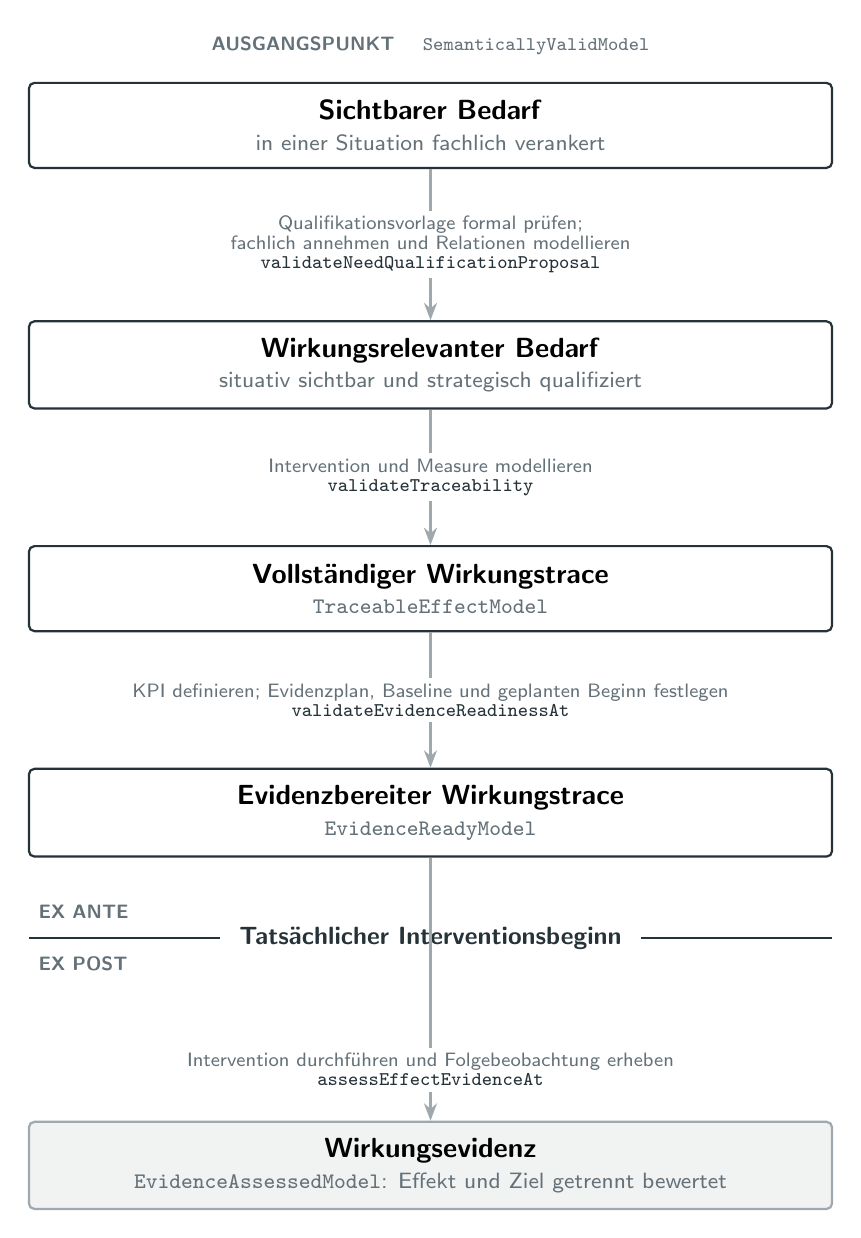
\begin{tikzpicture}[
  state/.style={
    draw=oink,
    fill=white,
    line width=0.8pt,
    rounded corners=2pt,
    minimum width=10.2cm,
    minimum height=1.08cm,
    align=center,
    inner sep=6pt,
    font=\sffamily
  },
  final state/.style={state, draw=oaccent, fill=osoft},
  flow/.style={-{Stealth[length=2.2mm]}, draw=oaccent, line width=1pt},
  gate/.style={
    fill=white,
    align=center,
    inner xsep=5pt,
    inner ysep=2pt,
    text=oink,
    font=\sffamily\scriptsize
  },
  phase/.style={font=\sffamily\scriptsize\bfseries, text=omuted}
]

\node[state] (visible) {
  \textbf{Sichtbarer Bedarf}\\[-1pt]
  {\footnotesize\color{omuted}in einer Situation fachlich verankert}
};
\node[phase, above=0.22cm of visible] {
  AUSGANGSPUNKT \quad \texttt{SemanticallyValidModel}
};

\node[state, below=1.92cm of visible] (relevant) {
  \textbf{Wirkungsrelevanter Bedarf}\\[-1pt]
  {\footnotesize\color{omuted}situativ sichtbar und strategisch qualifiziert}
};

\draw[flow] (visible) -- node[gate] {
  {\color{omuted}Qualifikationsvorlage formal prüfen;}\\[-1pt]
  {\color{omuted}fachlich annehmen und Relationen modellieren}\\[-1pt]
  \texttt{validateNeedQualificationProposal}
} (relevant);

\node[state, below=1.72cm of relevant] (traceable) {
  \textbf{Vollständiger Wirkungstrace}\\[-1pt]
  {\footnotesize\color{omuted}\texttt{TraceableEffectModel}}
};

\draw[flow] (relevant) -- node[gate] {
  {\color{omuted}Intervention und Measure modellieren}\\[-1pt]
  \texttt{validateTraceability}
} (traceable);

\node[state, below=1.72cm of traceable] (ready) {
  \textbf{Evidenzbereiter Wirkungstrace}\\[-1pt]
  {\footnotesize\color{omuted}\texttt{EvidenceReadyModel}}
};

\draw[flow] (traceable) -- node[gate] {
  {\color{omuted}KPI definieren; Evidenzplan, Baseline und geplanten Beginn festlegen}\\[-1pt]
  \texttt{validateEvidenceReadinessAt}
} (ready);

\coordinate[below=1.02cm of ready] (boundary);
\draw[oink, line width=0.9pt]
  ([xshift=-5.1cm]boundary) -- ([xshift=5.1cm]boundary);
\node[fill=white, inner xsep=7pt, font=\sffamily\small\bfseries, text=oink]
  at (boundary) {Tatsächlicher Interventionsbeginn};
\node[phase, anchor=south west]
  at ([xshift=-5.1cm,yshift=0.12cm]boundary) {EX ANTE};
\node[phase, anchor=north west]
  at ([xshift=-5.1cm,yshift=-0.12cm]boundary) {EX POST};

\node[final state, below=2.32cm of boundary] (assessed) {
  \textbf{Wirkungsevidenz}\\[-1pt]
  {\footnotesize\color{omuted}\texttt{EvidenceAssessedModel}: Effekt und Ziel getrennt bewertet}
};

\draw[flow] (ready) -- (boundary) -- node[gate, pos=0.72] {
  {\color{omuted}Intervention durchführen und Folgebeobachtung erheben}\\[-1pt]
  \texttt{assessEffectEvidenceAt}
} (assessed);

\end{tikzpicture}
\end{document}
